% !TEX root = ../main.tex


\chapter{Implementierung}
\label{ch:imp}

In diesem Kapitel wird die Umsetzung der in Kapitel~\ref{ch:KuD} definierten Konzepte und Designentscheidungen für das Framework im Detail beschrieben. Die Implementierung erfolgt als Erweiterung des bestehenden ArchitekturTools und nutzt dessen etablierten Technologie-Stack.

Zunächst wird die Backend-Implementierung vorgestellt, die sowohl die \gls{api} zur Verwaltung der Algorithmen als auch die Engine zur Ausführung der Validierungsläufe enthält. Danach wird die Implementierung der \gls{gui} erläutert, welche die Komponenten zur Algorithmenverwaltung und zur Visualisierung der Ergebnisse beinhaltet. Abschließend wird die Implementierung des ersten Validierungsalgorithmus erläutert, dessen Durchführung im Rahmen der Evaluation als \gls{poc} für die Funktionsfähigkeit des Frameworks dient.

\section{Backend}
\label{sec:backendimp}

Das Backend bildet den serverseitigen Kern des implementierten Frameworks. Es ist dabei für die zentrale Logik verantwortlich und setzt die zuvor entworfenen Konzepte für  Verwaltung und Steuerung um. Die Implementierung basiert auf der Node.js-Laufzeitumgebung in Verbindung mit dem Express.js-Framework und dem Prisma ORM. Die folgenden Unterabschnitte erläutern im Detail, wie sowohl zuvor konzipierte \gls{api} zur Algorithmenverwaltung als auch die Validierungsengine umgesetzt wurden.

\subsection{Umsetzung der API}
\label{subsec:api}

Um dem Frontend die Interaktion und Verwaltung der Validierungsalgorithmen zu ermöglichen, wurde serverseitig eine \gls{rest}-\gls{api} implementiert, die Endpunkte für alle erforderlichen CRUD-Operationen bereitstellt. Die neu implementierten Endpunkte integrieren sich in die bestehende Routing-Struktur des ArchitekturTools und sind unter dem Präfix \texttt{/api/v2/} erreichbar.

\subsubsection*{CREATE - \texttt{POST /api/v2/algorithm}}

Zum Anbinden neuer Validierungsalgorithmen dient der \texttt{POST}-Endpunkt. Zunächst wird ein ankommender Request von der \textit{Multer}\footnote{https://www.npmjs.com/package/multer}-Middleware verarbeitet, welche die hochgeladene Datei aus der \texttt{multipart/form-data}-Request extrahiert und in dem vordefinierten Verzeichnis (\texttt{/uploads/algorithm}) serverseitig speichert. Die Eindeutigkeit der Algorithmen wird gewährleistet, in dem vor dem Speichern mit der von Prisma zur Verfügung gestellten Methode \texttt{prisma\_db.algorithm.findFirst()} geprüft, ob ein Algorithmus mit dem übergebenen Namen bereits in der \texttt{algorithm}-Datenbanktabelle existiert. Falls dies der Fall ist, wird der Request mit dem Statuscode 409 Conflict abgelehnt. Andernfalls werden die Metadaten zusammen mit dem Dateipfad durch \texttt{prisma\_db.algorithm.create()} in der Datenbanktabelle abgelegt und der neu erstellte Datensatz mit dem Created-Statuscode als \textit{Response} zurückgegeben.

\subsubsection*{READ - \texttt{GET /api/v2/algorithms}}

Um alle verfügbaren Algorithmen im Frontend darzustellen, stellt der \texttt{GET}-Endpunkt eine Liste aller Einträge innerhalb der \texttt{algorithm}-Tabelle bereit. Dies wird durch den Aufruf der Prisma-Methode \texttt{prisma\_db.algorithm.findMany()} umgesetzt, die alle Datensätze abruft und als JSON-Array an das Frontend übermittelt.

\subsubsection*{UPDATE - \texttt{PATCH /api/v2/algorithm/:id}}

Zur Aktualisierung eines bestehenden Validierungsalgorithmus wird der \texttt{PATCH}-Endpunkt genutzt. Anhand der in der \textit{URL}\footnote{Uniform Resource Locator} übergebenen \texttt{:id} wird der zugehörige Datensatz mittels \texttt{prisma\_db.algorithm.findunique()} aus der \texttt{algorithm}-Tabelle abgerufen. Wird im Rahmen des Requests eine neue Datei hochgeladen, wird die alte, zugehörige Datei zunächst mit der Node.js-Funktion \texttt{fs.unlinkSync} vom Server gelöscht, um Dateien ohne Zugehörigkeit zu vermeiden. Anschließend werden die aktualisierten Metadaten sowie der neue Dateipfad mithilfe von \texttt{prisma\_db.\\ algorithm.update()} in der \texttt{algorithm}-Tabelle gespeichert.

\subsubsection*{DELETE - \texttt{DELETE /api/v2/algorithm/:id}}

Der \texttt{DELETE}-Endpunkt dient dem vollständigen Löschen eines Algorithmus. Um die Konsistenz des Systems sicherzustellen, folgt die Implementierung dieses Endpunkts einem zweistufigen Prozess: Zu Beginn wird der Datensatz anhand der übergebenen \texttt{:id} aus der Datenbank gelesen, um den Pfad zur entsprechenden Datei zu ermitteln. Diese Datei wird im Anschluss über \texttt{fs.promises.unlink} vom Dateisystem des Servers entfernt. Danach wird im zweiten Schritt der Datenbankeintrag selbst über \texttt{prisma\_db.algorithm.delete()} aus der Datenbanktabelle gelöscht. Mit diesem Ablauf wird sichergestellt, dass, wie beim \texttt{UPDATE}-Endpunkt, keine verwaisten Dateien auf dem Server zurückbleiben

\subsection{Integrierung der Validierungs-Engine}
\label{subsec:engine}

Die Durchführung der Validierungsläufe bildet die Schlüsselfunktionalität des Backends. Sie ist dafür zuständig die Daten aufzubereiten, die kontrollierte Ausführung eines isolierten Python-Prozessesund die sowie die Verarbeitung und Abspeicherung der Ergebnisse. Dieser Prozess wird durch einen dedizierten \gls{api}-Endpunkt gestartet.

Der komplette Ablauf eines Validierungslaufs, von der Aufbereitung der Daten über die Ausführung des isolierten Python-Prozess bis hinzur Speicherung des Ergebnisses, ist ein aufeinander abgestimmter Prozess. Abbildung~\ref{fig:seqvalid} verdeutlicht das Zusammenspiel der beteiligten Komponenten.

\begin{figure}[h!]
  \centering
  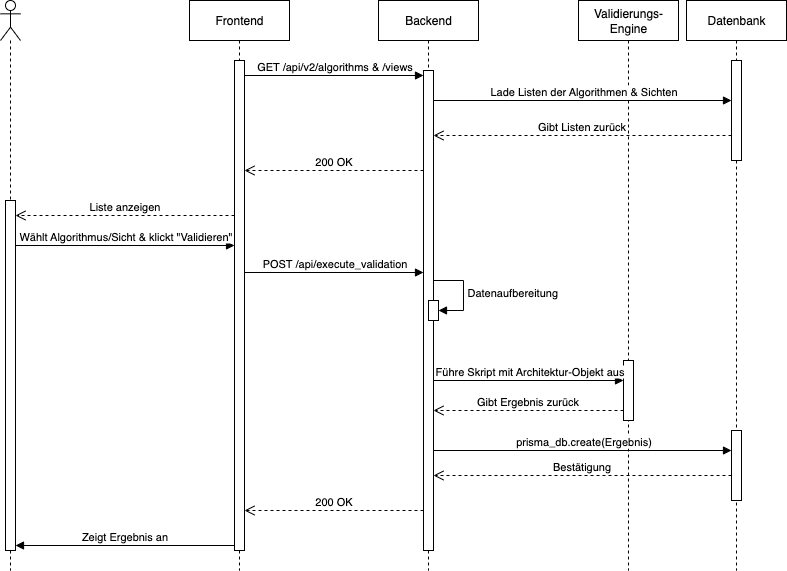
\includegraphics[width=\textwidth]{figures/05Implementierung/Sequenz_valid.drawio.png}
  \caption{Verlauf einer Architekturvalidierung im Framework}
  \label{fig:seqvalid}
\end{figure}

\subsubsection*{Datenaufbereitung und Export}

Nachdem der Request mit den IDs für den Algorithmus und der Architektursicht validiert wurde, stellt die Engine die erforderlichen Komponentendaten bereit. Hierfür wird auf eine angepasste Version des bestehenden \textit{JSON-Exporter} des ArchitekturTool zurückgegriffen.

Die Engine prüft zunächst, ob die Komponenten der angeforderten Sicht bereits als Datei im JSON-Format auf dem Server liegen. Falls nicht, wird der Exportprozess automatisch gestartet, welcher die Komponentendaten aus der Datenbank extrahiert und in einem sichten-spezifischen Ordner abgelegt. Anschließend werden diese JSON-Dateien eingelesen und zu einem einzigen Architektur-Objekt zusammengefügt, das als Eingabe für den Validierungsalgorithmus dient.

\subsubsection*{Durchführung des Python-Prozess}

Die eigentliche Validierung wird in einem isolierten Python-Prozess durchgeführt, um die Stabilität des Servers zugewährleisten. Hierfür wird die \texttt{spawn}-Funktion aus dem \texttt{child\_process}-Modul von Node.js genutzt. Diese startet das Python-Skript, das zum ausgewählten Algorithmus gehört. Das zuvor erstellte Architektur-Objekt wird als JSON-String in den Standard-Input des Python-Prozesses geschrieben. Eventuelle Probleme beim Starten des Prozesses werden vom Error-Listener abgefangen.

\subsubsection*{Ergebnisverarbeitung}

Gegen Ende der Durchführung nimmt das Backend die Standardausgabe und die Fehlerausgabe des Python-Skripts entgegen. Wenn ein Fehler auftretet, wird der Validierungslauf als fehlgeschlagen gewertet und ein entsprechender Eintrag mit der entsprechenden Fehlermeldung in der \texttt{result}-Tabelle der Datenbank gespeichert. Anhand der Definierung der Struktur des Objekts wird der Ergebnistyp dynamisch als \texttt{TEXT} oder \texttt{METRIC} bestimmt. Schließlich wird das Ergebnis gemeinsam mit den Metadaten wie der Ausführungsdauer und dem Erfolgsstatus mithilfe von Prisma auch in der \texttt{result}-Tabelle abgespeichert und zur Visualisierung an das Frontend gesendet.

\section{Frontend}
\label{sec:frontendimp}

Die \gls{gui} wurde mit React entwickelt und folgt einer modularen, komponentenbasierten Architektur, was eine klare Trennung der Zuständigkeit ermöglicht. Ein übergeordneter \texttt{ValidationContainer} verwaltet den gesamten Anwendungszustand wie Ladeindekatoren, Fehler, Ergebnisse und Validierungsverlauf. Dieser Zustandshalter gibt Daten sowie Callback-Funktion über Props an  die untergeordneteten Komponennten weiter. Zur Speicherung des Verlaufs über die Browsersitzung hinweg nutzt der Zustandshalter den \texttt{localStorage} des Browser.

\subsection{Algorithmenverwaltungs-Komponenten}
\label{subsec:verwaltung}

Die Verwaltung der Algorithmen ist die zentrale Interaktionsstelle für den Nutzer. Diese besteht aus einer Hauptkomponente zur Steuerung und einem modalen Fenster zum Erstellen, Bearbeiten und Löschen der Algorithmen.

\subsubsection*{Hauptkomponente}

Die zentrale Steuereinheit ruft bei ihrer Initialisierung mithilfe der Lebenszyklus-Methode \texttt{componentDidMount} über \textit{axios}\footnote{https://axios-http.com/docs/intro} asynchron jeweils die \texttt{GET}-Request die Algorithmen und die Architektursichten auf. Die erhaltenen Daten werden lokal im Zustand der Komponente gespeichert und dazu genutzt, die beiden Auswahllisten zu füllen. Die \texttt{onChange}-Handler dieser Listen aktualisieren den Zustand, sobald ein Algorithmus bzw. eine Sicht ausgewählt wurde.

Ein Klick auf den deidzierten \glqq Validieren\grqq{}-Button startet den in Abschnitt~\ref{subsec:engine} beschriebenen Validierungslauf. Dabei wird eine \texttt{POST}-Request mit der \texttt{algorithmId} und \texttt{viewId} als Parameter an den entsprechenden Endpunkt gesendet. Mittels einer Callback-Funktion wird der Fortschritt und das Ergebnis dieses Durchlaufs an die übergeordnete Container-Komponente gesendet.

\subsubsection*{Modalfenster}

Für das Hochladen, Bearbeiten und Entfernen der Algorithmen wird die Komponente \texttt{AlgorithmModal} genutzt die ein seperates Fenster öffnet. Dieses modale Fenster unterscheidet zwischen einem Hochladungs- und einem Bearbeitungsmodus, je nachdem, ob eine \texttt{selectedAlgorithm}-Prop übergeben wird. Im Bearbeitungsmodus wird das Formular bereits mit den jeweiligen Daten vorbefüllt.Dem Nutzer wird es mithilfe des integrierten \textit{Monaco-Editors}\footnote{https://microsoft.github.io/monaco-editor/} ermöglicht, Python-Code direkt im Browser zu schreiben, einzufügen und zu bearbeiten. Um dem Nutzer dabei den Einstieg zu erleichtern und die Konsistenz der Algorithmen zu gewährleisten, wird ein Code-Gerüst als Vorlage bereitgestellt, wie in Abbildung~\ref{fig:codeskeleton} dargestellt.

Die Ziele beim Anbinden neuer Algorithmen sind das vereinfachen und das standardisieren:

\begin{itemize}
  \item \textbf{Verringern von Boilerplate-Code:} Das Gerüst enthält eine \texttt{main}-Funktion, welche die gesamte Interaktion mit der Engine zusammenfasst. Sie übernimmt das einlesen der Architektur über den Input, die Fehlerbehandlung bei ungültigem JSON sowie das Schreiben des Ergebnis-Objekts auf den Output. Nutzer müssen sich somit nicht mit dem wiederkehrenden Teil des Codes befassen.
  \item \textbf{Klar definierter Bereich:} Durch die vorgegebene Struktur, ist die einzige Aufgabe des Nutzers, die Funktion \texttt{run\_validation\_algorithm} mit der eigentlich Validierung zu füllen. Somit wird sichergestellt, das der Fokus nur auf das Prüfen der Logik liegt.
  \item \textbf{Bereitstellung gängiger Bibliotheken:} Wie in Abbildung~\ref{fig:codeskeleton} zu sehen ist, importiert das Gerüst bereits einige in der Architekturvalidierung etablierten Bibliotheken, darunter \texttt{pandas, numpy, matplotlib} und \texttt{cantools}. Damit wird eine einheitliche und leistungsstarke Entwicklungsumgebung geschaffen. Natürlich kann man manuell weitere Bibliotheken hinzufügen, indem man diese in der \texttt{py-libraries.txt} hinein schreibt.
  \item \textbf{Definierte Ergebnisstruktur:} Das Gerüst gibt durch die Dokumentation eine klare Struktur für das Ergebnis-Dictionary vor. Der Nutzer legt durch die Wahl der Schlüsselbegriffe im zurückgegebenen Dictionary fest, wie das Ergebnis zu interpretieren ist. Diese Struktur ist entscheidend, da sie vom Backend ausgelesen wird, um den Typen des Ergebnisses (\texttt{TEXT} oder \texttt{METRIC}). zu bestimmen. Damit wird es dem Frontend ermöglicht, ohne weitere Konfiguration die passende Visualisierungskomponente zu wählen.
\end{itemize}

Beim Speichern wird der Code aus dem Editor in ein \texttt{Blob}- und anschließend in eine \texttt{File}-Objekt umgewandelt. Dieses wird zusammen mit den Metadaten aus dem Formular über eine \texttt{POST}- oder \texttt{PATCH}-Request an das Backend gesendet. Zusätzlich ist eine Löschfunktion implementiert, welche mit einer \texttt{DELETE}-Request die entsprechenden Einträge entfernt.

Der vollständige Prozess des Anbinden eines Validierungsalgorithmus, von der Eingabe des Nutzers im Modalfenster bis zum finalen speichern, wird in Abbildung~\ref{fig:anbindung} als Sequenzdiagramm veranschaulicht.

\begin{figure}[h!]
  \centering
  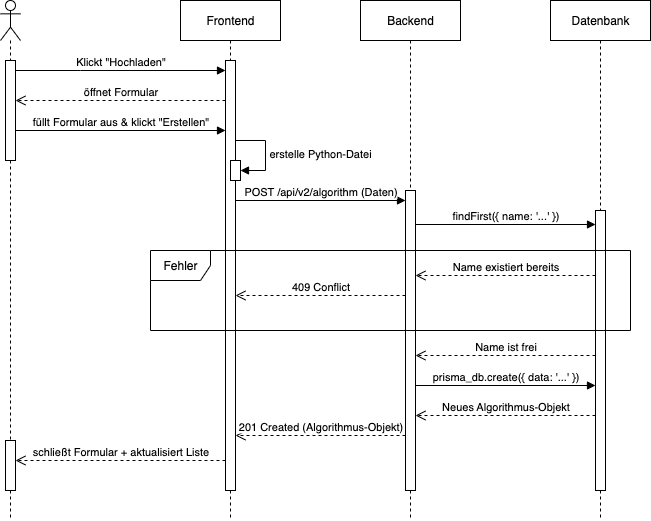
\includegraphics[width=\textwidth]{figures/05Implementierung/Sequenz_Algo_erstellen.drawio.png}
  \caption{Anbindungsprozess innerhalb des Validierungs-Frameworks}
  \label{fig:anbindung}
\end{figure}

Wie in der Abbildung dargestellt, wird vom Frontend aus ein \texttt{POST}-Request an das Backend gesendet. Dabei ist ein wichtiger Aspekt die anschließende Prüfung auf einen Namenskonflikt, bevor der neue Datensatz in der Datenbank abgespeichert wird.
\subsection{Visualisierung der Ergebnisse}
\label{subsec:visual}
Die Darstellung der Ergebnisse ist, ebenso wie die Algorithmenverwaltung, modular aufgebaut, um verschiedene Ergebnistypen und eine Ergebnishistorie abzubilden. Sie unterteilt sich in die dynamische Darstellung des aktuellen Ergebnisses, mit der zugrundeliegenden Graphenvisualisierung und dem Verlauf der Validierungsdurchläufe.

Mithilfe dieser Komponente wird das Validierungsergebnis der aktuellen Ausführung visualisiert. Ihr gerenderter Inhalt wird durch die vom Container übergebenen Props gesteuert.

Das Kernstück dieser Komponente ist das dynamische Rendern der Ergebnisse, das auf den \texttt{resultType}-Prop basiert. Hier wird mittels \texttt{switch}-Anweisung, je nach Ergebnistyp, die passende Visualisierung ausgewählt:

\begin{itemize}
  \item \textbf{Textuelle Ausgabe(\texttt{TEXT}):} Standardmäßig werden die Ergebnisse als JSON in einem \texttt{<pre>}-Element dargestellt. Wie dieser formatiert sein soll bestimmt der Nutzer in seinem Python-Code.
  \item \textbf{Metrische Ausgabe(\texttt{METRIC}):} Bei metrischen Ergebnisdaten wird die Komponente Diagramm-Visualisierung instanziiert. Ihr werden die Messwerte und Grenzwerte als Props übergeben, woraufhin die Komponente die Darstellung als Linien-, Balken- oder Flächendiagramm übernimmt.
\end{itemize}

Der Ansatz des dynamischen Rendern stellt sicher, dass das Frontend flexibel auf unterschiedliche Ausgabeformate der Algorithmen reagieren kann, ohne dass Änderungen an der Komponente vorgenommen werden müssen.

\subsubsection*{Diagramm-Visualisierung}

Die Visualisierung der metrischen Daten baut auf der populären Bibliothek \textit{Recharts}\footnote{https://recharts.org/en-US}, welche mit den gelieferten Daten in eine interaktive und auswertbare grafische Form überführt (Siehe Abbildung~\ref{fig:metricvis}).

Der Ablauf innerhalb dieser Komponente ist wie folgt:

\begin{enumerate}
  \item \textbf{Normalisierung der Daten:} Zunächst werden die eingehenden Daten durch eine Funktion aufbereitet und normalisiert. Diese Funktion extrahiert aus den Datenpunkten eine einheitliche Bezeichnung für die X-Achse, welche entweder aus einem \texttt{timestamp} oder \texttt{name} Feld entnommen wird. Außerdem stellt sie sicher, dass die restlichen numerischen Werte korrekt als verwertbare Datenserie für das Diagramm zur Verfügung stehen.
  \item \textbf{Dynamische Diagramm-Auswahl:} Basierend auf dem\texttt{chartType}-Prop, die vom Validierungsalgorithmus mit dem Ergebnis-Dictionary mitgegeben wird, wählt die Komponente dynamisch die passende Visualisierung aus Recharts aus (\texttt{LineChart, BarChart} oder \texttt{AreaChart}). Dies ermöglicht dem Ersteller des Algorithmus, die am besten geeignete Darstellungsform für die Metrik vorzugeben.
  \item \textbf{Visualisierung von Grenzwerten:}Ein wichtiges Feature ist es Grenzwerte visuell darzustellen. Wird ein \texttt{threshold} übergeben, rendert die Komponente eine horizontale, gestrichelte Linie in das Diagramm. Dies macht es sofort ersichtlich, ob die Messwerte innerhalb des erwarteten Bereichs liegen. Zudem wurde eine Funktion zur Prüfung jedes einzelnen Datenpunkt eines Liniendiagramms implementiert, welches man in Abbildung~\ref{fig:Liniendiagramm} gut erkennen kann. Wird der Wert des definierten Grenzwerts überschritten, wird der zugehörige Punkt innerhalb des Diagramms farblich markiert.
\end{enumerate}

\begin{figure}[h!]
  \centering
  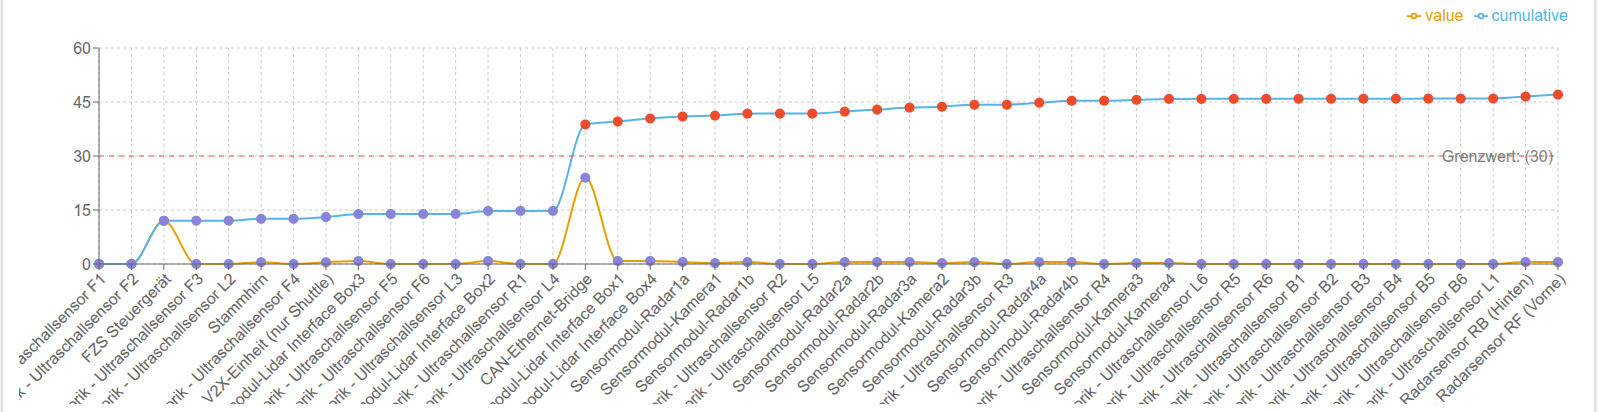
\includegraphics[width=\textwidth]{figures/06Evaluation/Line.png}
  \caption{Das Ergebnis als Liniendiagramm samt Grenzwert visualisiert}
  \label{fig:Liniendiagramm}
\end{figure}

Des Weiteren werden UI-Elemente, wie eine Legende, Tooltips beim überfahren mit der Maus sowie beschriftete X-,Y-Achsen, gerendert um eine hohe Benutzerfreundlichkeit und eine einfache Interpretation zu gewährleisten.

\subsubsection*{Eregbnishistorie}

Damit die Verfolgbarkeit der Validierungsergebenisse zu gewährleisten, wird die Komponente für die Darstellung der letzten Zehn Validierungsläufe implementiert. Hierzu wird die \texttt{history}-Prop vom übergeordneten Container empfangen, der diesen Zustand über den \texttt{localStorage}-Service des Webbrowsers auch nach einem Neuladen der Seiter erhält.

Die Ergebnisse werden hierbei in Form einer aufklappbaren Liste präsentiert, um die Benutzeroberfläche übersichtlich zu halten. Listeneinträge zeigen zunächst die wichtigsten Eckdaten bzgl. des Validierungslauf: Name des Algorithmus, die gewählte Architektursicht und dem Zeitstempel der Durchführung. Mit einem Klick auf den jeweiligen Eintrag öffnet sich dieser und visualisiert die vergangenen Ergebnisse mit der selben Darstellung wie bei der Visualisierung der aktuellen Ergebnisse. Dieser Ansatz stellt eine konsistente Nutzererfahrung sicher.
\section{Validierungsalgorithmus}
\label{sec:validimp}

Als \gls{poc} für das entwickelte Framework wird ein erster Validierungsalgorithmus implementiert. Bei dem zu realisierenden Algorithmus handelt es sich um einen Traceability-Check. Überprüfungen dieser Art sind während der Systementwicklungsphase von großer wichtigkeit, da sie die Nachverfolgbarkeit zwischen Anforderungen und deren Umsetzung Sicherstellen. Somit lassen sich Anforderungen ohne Umsetzungen sowie Garantien ohne Anforderungen aufdecken. Dabei handelt es sich um einen wichtigen Schritt, um die Vollständigkeit und Korrektheit einer Architektur zu beurteilen. Der Algorithmus wird in das Codegerüst, welches in Abschnitt~\ref{subsec:verwaltung} beschrieben wurde, integriert.

Der Algorithmus wird wie folgt implementiert:
\begin{enumerate}
  \item Zunächst werden alle Komponenten des Architektur-Objekts vom Algorithmus durchlaufen. Dabei werden alle Anforderungen und Garantien in zwei verschiedenen Dictionaries gespeichert. Dies ermöglicht später einen effizienten Zugriff und einfache Nachverfolgung der Verbindungen zwischen den beiden.
  \item Danach werden die gesammelten Daten untersucht. Es werden vier Listen erstellt, in die jeweils Anforderungen und Garantien wie folgt einsortiert werden:
        \begin{itemize}
          \item Anforderungen mit zugeordenten Garantien
          \item Anforderungen ohne zugeordnete Garantien
          \item Garantien mit zugeordneten Anforderungen
          \item Garantien ohne zugeordnete Anforderungen
        \end{itemize}
  \item Abschließend wird mithilfe diesen vier Listen ein Report erstellt, welcher lesbar und einfach zu verstehen ist. Für jeden Abschnitt werden die entsprechenden Elemente aufgelistet und formartiert, wodurch der Nutzer auf einen Blick erkennen kann, welche Anforderungen noch nicht umgesetzt wurden oder welche Garantien noch keine Anforderung erfüllen.
\end{enumerate}

Im folgenden Kapitel dient dieser Algorithmus als konkreter Anwendungsfall zur Evaluation des Frameworks. Durch seine Ausführung wird die Funktionsfähigkeits der Erweiterungen nachgewiesen.